% Generated by paper/build_parameter_figures.py; do not hand edit.
% Source: CURRENT_RESULTS_TABLES.md; normalized SHA-256 babf158f4e596c41a220fcc2993a466fc538dc0758ddf9f78e6d62741be570e6
% Rounded binary64 diagnostics, not new outward-rounded certificates.
\begin{figure}[tb]
\centering
\begin{minipage}[t]{.485\linewidth}\begin{minipage}[t]{\linewidth}
\centering
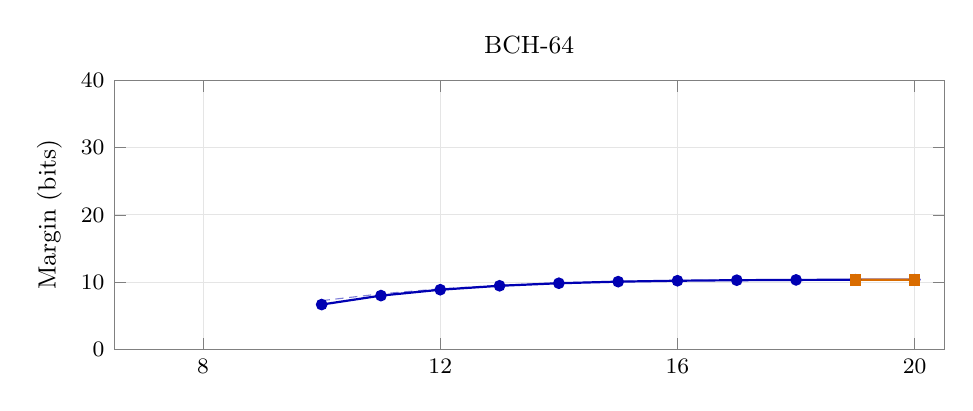
\begin{tikzpicture}
\begin{axis}[tick label style={font=\footnotesize},label style={font=\small},title style={font=\small},grid=major,grid style={black!10},axis line style={black!50},legend style={font=\footnotesize,draw=none},width=\linewidth,height=5.0cm,title={BCH-64},xmin=6.5,xmax=20.5,ymin=0,ymax=40,xtick={8,12,16,20},ytick={0,10,20,30,40},ylabel={Margin (bits)},]
\addplot[blue!70!black,thick,mark=*,mark size=1.7pt,unbounded coords=jump] coordinates {(7,nan) (8,nan) (9,nan) (10,6.674265000) (11,8.004586000) (12,8.880604000) (13,9.464553000) (14,9.842649000) (15,10.077023000) (16,10.215546000) (17,10.293941000) (18,10.336863000) (19,10.359841000) (20,10.371924000)};
\addplot[blue!70!black,densely dashed,opacity=.5,unbounded coords=jump,forget plot] coordinates {(7,nan) (8,nan) (9,nan) (10,7.258641000) (11,8.269308000) (12,9.013821000) (13,9.539167700) (14,9.889113100) (15,10.108979400) (16,10.239631800) (17,10.313623400) (18,10.354056000) (19,10.375636200) (20,10.386947400)};
\addplot[orange!85!black,thick,mark=square*,mark size=1.7pt,unbounded coords=jump] coordinates {(8,nan) (9,nan) (10,nan) (11,nan) (12,nan) (13,nan) (14,nan) (15,nan) (16,nan) (17,nan) (18,nan) (19,10.353300000) (20,10.365380000)};
\addplot[orange!85!black,densely dashed,opacity=.5,unbounded coords=jump,forget plot] coordinates {(8,nan) (9,nan) (10,nan) (11,nan) (12,nan) (13,nan) (14,nan) (15,nan) (16,nan) (17,nan) (18,nan) (19,10.369172800) (20,10.380476100)};
\end{axis}
\end{tikzpicture}
\end{minipage}

\par
\begin{minipage}[t]{\linewidth}
\centering
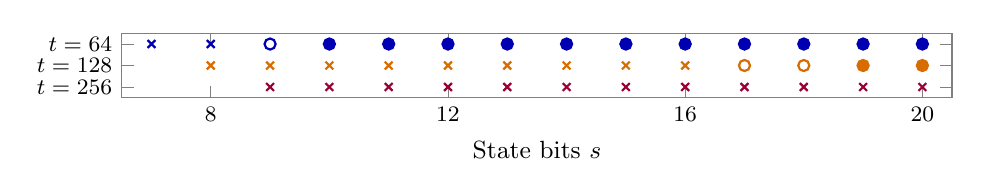
\begin{tikzpicture}
\begin{axis}[tick label style={font=\footnotesize},label style={font=\small},title style={font=\small},grid=major,grid style={black!10},axis line style={black!50},legend style={font=\footnotesize,draw=none},width=\linewidth,height=2.4cm,xmin=6.5,xmax=20.5,ymin=.5,ymax=3.5,xtick={8,12,16,20},xlabel={State bits $s$},ytick={1,2,3},yticklabels={$t=256$,$t=128$,$t=64$},grid=none,]
\addplot[only marks,blue!70!black,mark=*,mark size=2pt,thick] coordinates {(10,3.000000000) (11,3.000000000) (12,3.000000000) (13,3.000000000) (14,3.000000000) (15,3.000000000) (16,3.000000000) (17,3.000000000) (18,3.000000000) (19,3.000000000) (20,3.000000000)};
\addplot[only marks,blue!70!black,mark=o,mark size=2pt,thick] coordinates {(9,3.000000000)};
\addplot[only marks,blue!70!black,mark=x,mark size=2pt,thick] coordinates {(7,3.000000000) (8,3.000000000)};
\addplot[only marks,orange!85!black,mark=*,mark size=2pt,thick] coordinates {(19,2.000000000) (20,2.000000000)};
\addplot[only marks,orange!85!black,mark=o,mark size=2pt,thick] coordinates {(17,2.000000000) (18,2.000000000)};
\addplot[only marks,orange!85!black,mark=x,mark size=2pt,thick] coordinates {(8,2.000000000) (9,2.000000000) (10,2.000000000) (11,2.000000000) (12,2.000000000) (13,2.000000000) (14,2.000000000) (15,2.000000000) (16,2.000000000)};
\addplot[only marks,purple!80!black,mark=x,mark size=2pt,thick] coordinates {(9,1.000000000) (10,1.000000000) (11,1.000000000) (12,1.000000000) (13,1.000000000) (14,1.000000000) (15,1.000000000) (16,1.000000000) (17,1.000000000) (18,1.000000000) (19,1.000000000) (20,1.000000000)};
\end{axis}
\end{tikzpicture}
\end{minipage}
\end{minipage}\hfill
\begin{minipage}[t]{.485\linewidth}\begin{minipage}[t]{\linewidth}
\centering
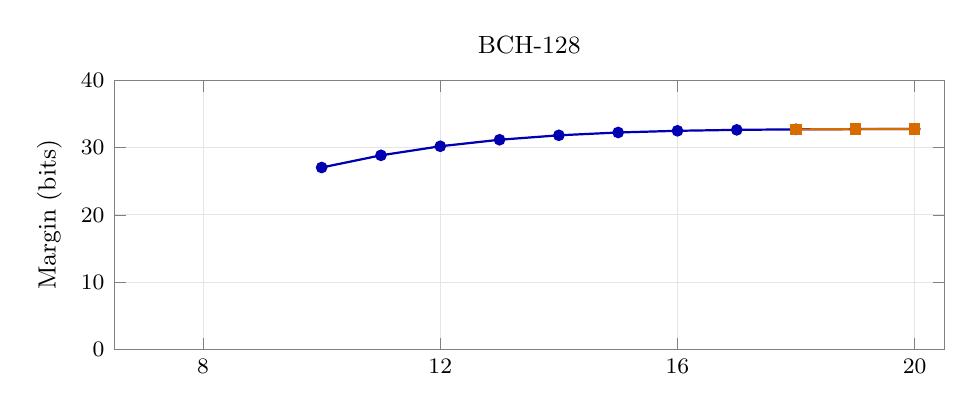
\begin{tikzpicture}
\begin{axis}[tick label style={font=\footnotesize},label style={font=\small},title style={font=\small},grid=major,grid style={black!10},axis line style={black!50},legend style={font=\footnotesize,draw=none},width=\linewidth,height=5.0cm,title={BCH-128},xmin=6.5,xmax=20.5,ymin=0,ymax=40,xtick={8,12,16,20},ytick={0,10,20,30,40},ylabel={Margin (bits)},]
\addplot[blue!70!black,thick,mark=*,mark size=1.7pt,unbounded coords=jump] coordinates {(7,nan) (8,nan) (9,nan) (10,27.041016000) (11,28.850828000) (12,30.197059000) (13,31.166105000) (14,31.824891000) (15,32.244724000) (16,32.494912000) (17,32.635244000) (18,32.710487000) (19,32.749575000) (20,32.769598000)};
\addplot[blue!70!black,densely dashed,opacity=.5,unbounded coords=jump,forget plot] coordinates {(7,nan) (8,nan) (9,nan) (10,27.041018141) (11,28.850828493) (12,30.197059153) (13,31.166105060) (14,31.824891029) (15,32.244724017) (16,32.494912011) (17,32.635244008) (18,32.710487007) (19,32.749575006) (20,32.769598006)};
\addplot[orange!85!black,thick,mark=square*,mark size=1.7pt,unbounded coords=jump] coordinates {(8,nan) (9,nan) (10,nan) (11,nan) (12,nan) (13,nan) (14,nan) (15,nan) (16,nan) (17,nan) (18,32.699951000) (19,32.739117000) (20,32.759209000)};
\addplot[orange!85!black,densely dashed,opacity=.5,unbounded coords=jump,forget plot] coordinates {(8,nan) (9,nan) (10,nan) (11,nan) (12,nan) (13,nan) (14,nan) (15,nan) (16,nan) (17,nan) (18,32.699951007) (19,32.739117006) (20,32.759209006)};
\end{axis}
\end{tikzpicture}
\end{minipage}

\par
\begin{minipage}[t]{\linewidth}
\centering
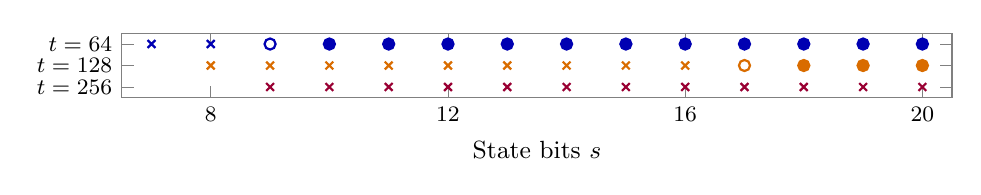
\begin{tikzpicture}
\begin{axis}[tick label style={font=\footnotesize},label style={font=\small},title style={font=\small},grid=major,grid style={black!10},axis line style={black!50},legend style={font=\footnotesize,draw=none},width=\linewidth,height=2.4cm,xmin=6.5,xmax=20.5,ymin=.5,ymax=3.5,xtick={8,12,16,20},xlabel={State bits $s$},ytick={1,2,3},yticklabels={$t=256$,$t=128$,$t=64$},grid=none,]
\addplot[only marks,blue!70!black,mark=*,mark size=2pt,thick] coordinates {(10,3.000000000) (11,3.000000000) (12,3.000000000) (13,3.000000000) (14,3.000000000) (15,3.000000000) (16,3.000000000) (17,3.000000000) (18,3.000000000) (19,3.000000000) (20,3.000000000)};
\addplot[only marks,blue!70!black,mark=o,mark size=2pt,thick] coordinates {(9,3.000000000)};
\addplot[only marks,blue!70!black,mark=x,mark size=2pt,thick] coordinates {(7,3.000000000) (8,3.000000000)};
\addplot[only marks,orange!85!black,mark=*,mark size=2pt,thick] coordinates {(18,2.000000000) (19,2.000000000) (20,2.000000000)};
\addplot[only marks,orange!85!black,mark=o,mark size=2pt,thick] coordinates {(17,2.000000000)};
\addplot[only marks,orange!85!black,mark=x,mark size=2pt,thick] coordinates {(8,2.000000000) (9,2.000000000) (10,2.000000000) (11,2.000000000) (12,2.000000000) (13,2.000000000) (14,2.000000000) (15,2.000000000) (16,2.000000000)};
\addplot[only marks,purple!80!black,mark=x,mark size=2pt,thick] coordinates {(9,1.000000000) (10,1.000000000) (11,1.000000000) (12,1.000000000) (13,1.000000000) (14,1.000000000) (15,1.000000000) (16,1.000000000) (17,1.000000000) (18,1.000000000) (19,1.000000000) (20,1.000000000)};
\end{axis}
\end{tikzpicture}
\end{minipage}
\end{minipage}
\caption{State and step size at $K=2^{20}$. Blue circles: $t=64$; orange
squares: $t=128$. Solid and faint dashed curves have the meanings in
Figure~\ref{fig:finite-k-b}. The strips below show every tested state:
filled dots denote useful full bounds, open circles weak full upper bounds,
and crosses a positive first-moment lower obstruction. No useful full curve
is available for $t=256$ (purple). Strip heights are categories, not margins.
An obstruction rules out a small first moment for that map, not the code's
distance property.}
\label{fig:finite-s-t}
\end{figure}
